% ...existing code...

\chapter{Web Application}

This chapter presents a simple Flask application connecting to the Oracle database. 
It employs multiple routes for the main operations:

\begin{itemize}
    \item \textbf{Order management.} Users can insert new orders (\texttt{/add\_order}) 
    and assign them to teams (\texttt{/assign\_order}).
    \item \textbf{Customer registration.} A new customer can be added (\texttt{/register\_customer}), 
    supporting both ''individual'' and ''business'' types.
    \item \textbf{Team statistics.} Routes like \texttt{/team\_stats} and \texttt{/teams\_list} 
    give information about total orders handled by a specific team, the total cost of the orders handled by a specific team and information about performance score of all teams.
\end{itemize}

The code centralizes database access in a separate \texttt{database.py} module. 
Each route follows the typical Flask pattern of ''GET to render form, POST to handle form input.'' 

Procedure and function calls (e.g., \texttt{registerCustomer}, \texttt{addOrder}, or \texttt{assignOrderToTeam}) are used to interact with the Oracle schema, ensuring logic remains in the PL/SQL layer.

\begin{figure}[H]
    \centering
    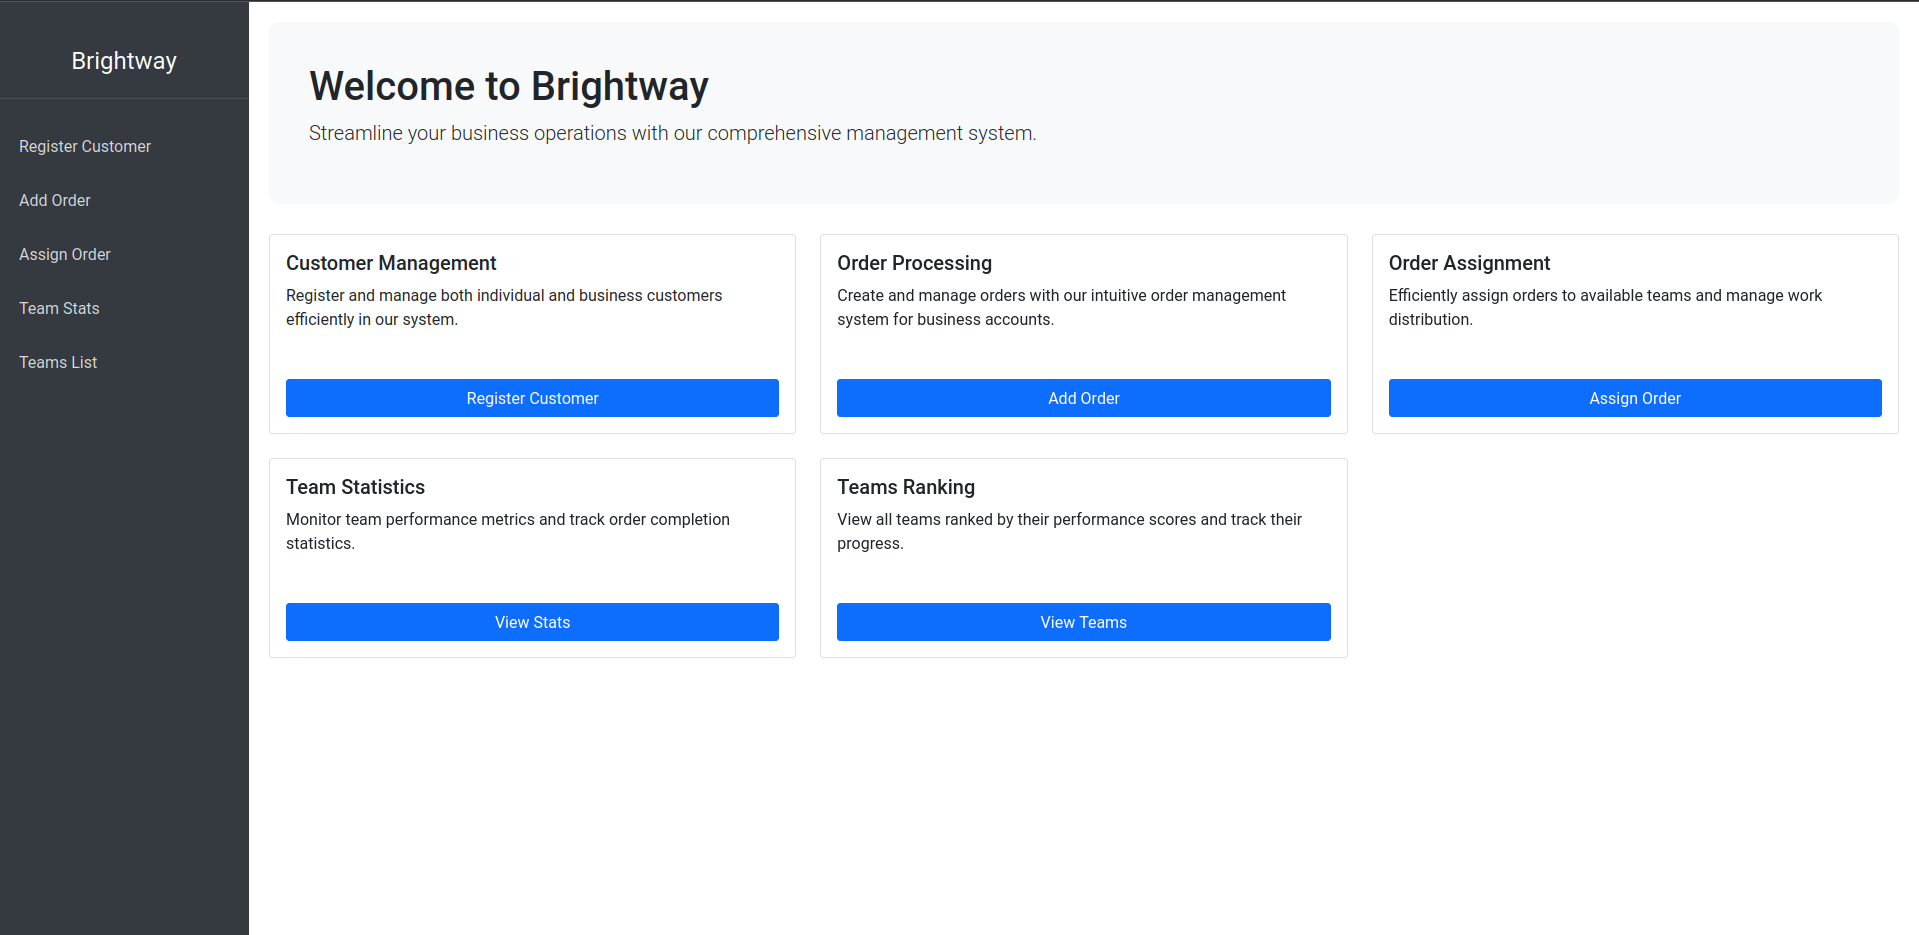
\includegraphics[width=0.8\textwidth]{img/web_app/home.png}
    \caption{Home page of the web application.}
\end{figure}

\begin{figure}[H]
    \centering
    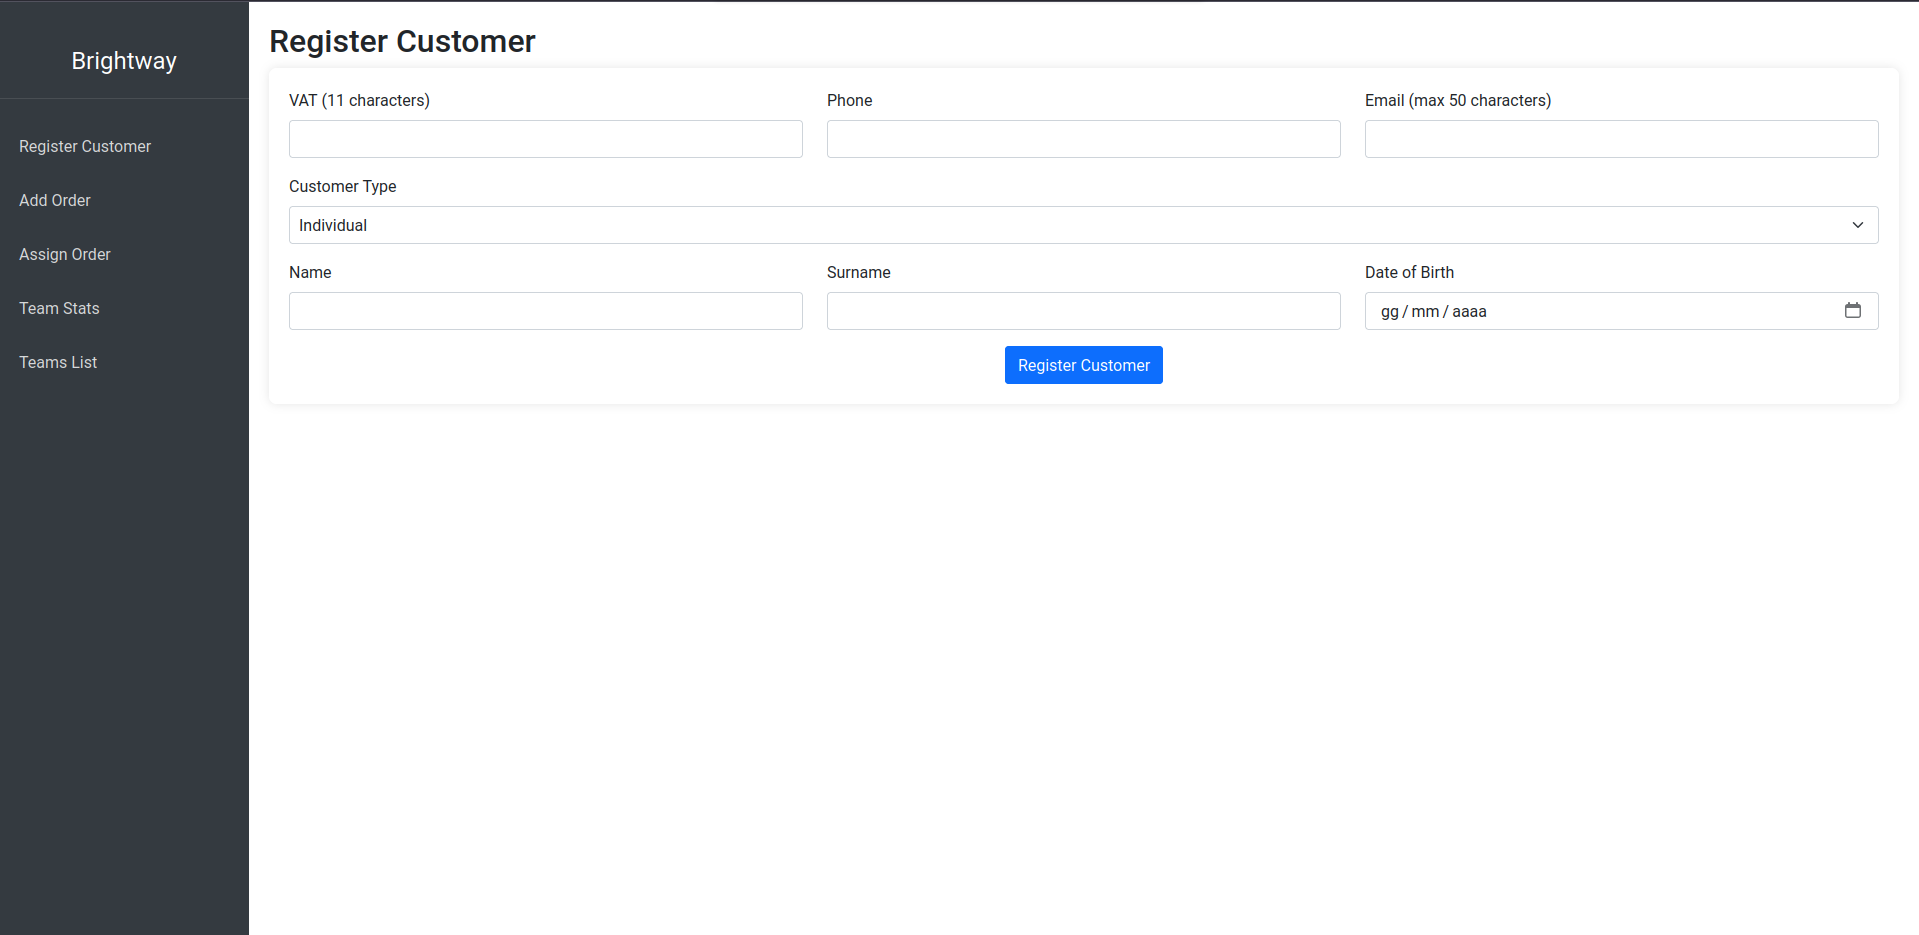
\includegraphics[width=0.8\textwidth]{img/web_app/customer_i.png}
    \caption{Customer registration form for individual customers.}
\end{figure}

\begin{figure}[H]
    \centering
    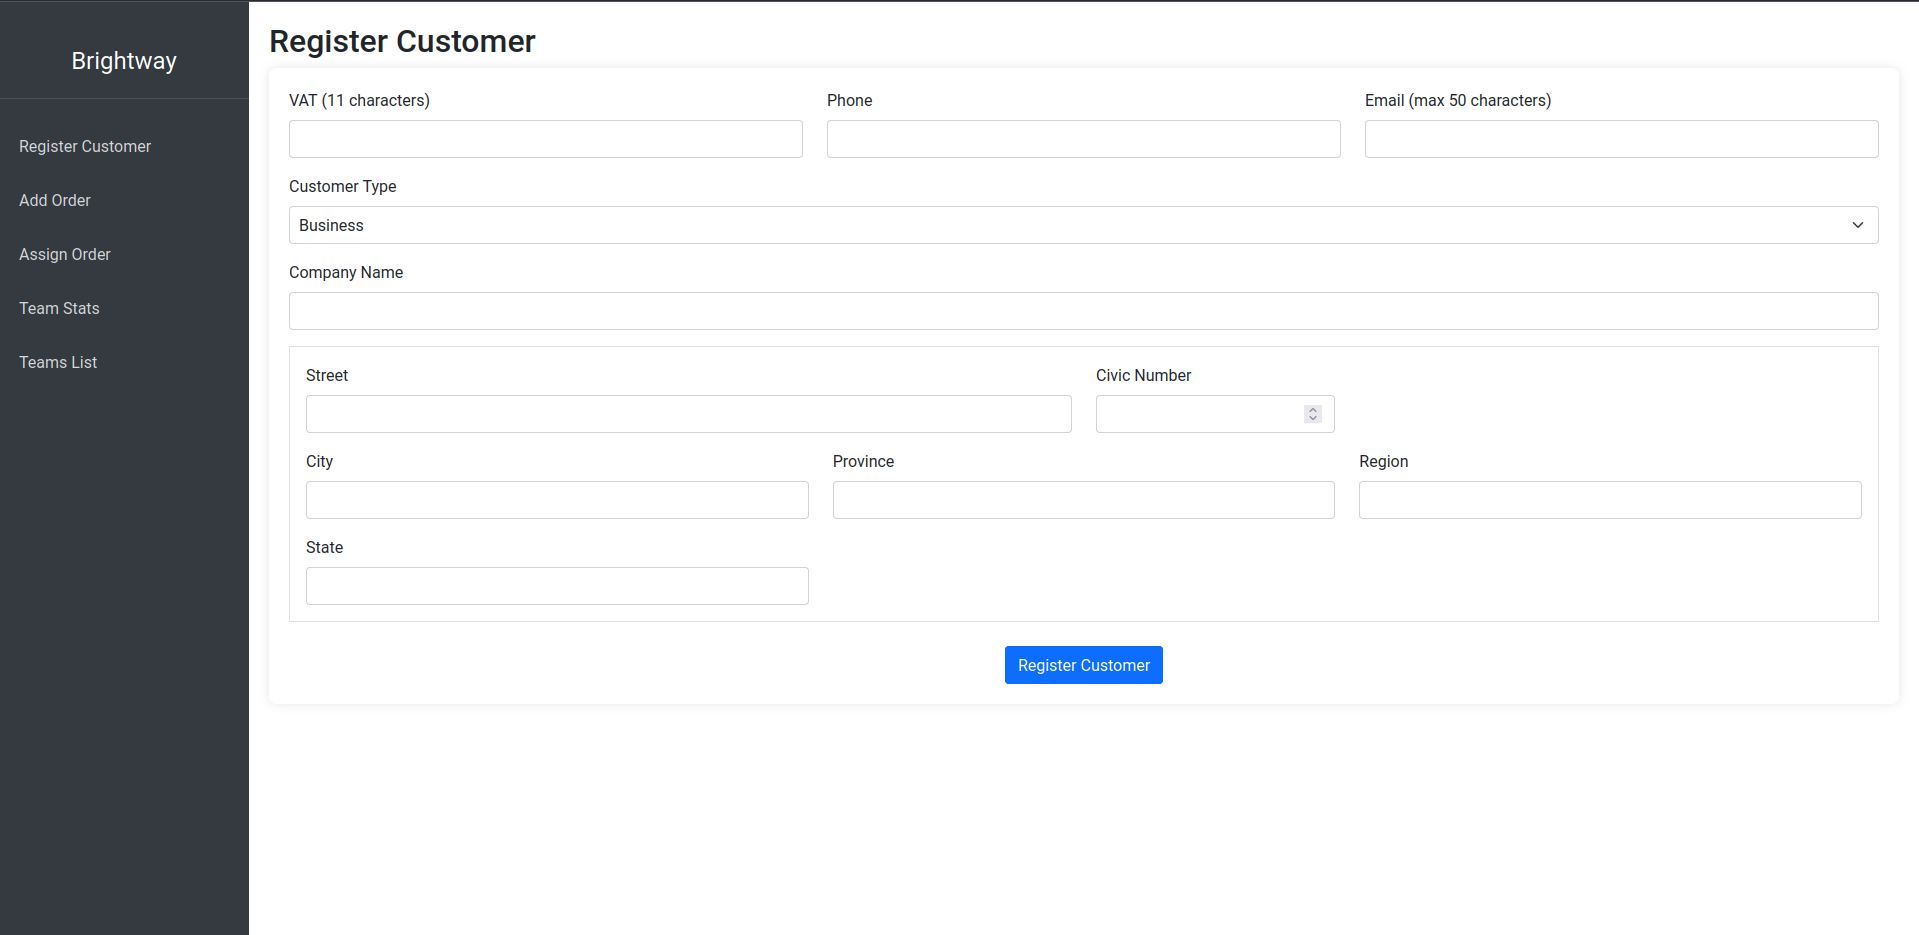
\includegraphics[width=0.8\textwidth]{img/web_app/customer_b.png}
    \caption{Customer registration form for business customers.}
\end{figure}

\begin{figure}[H]
    \centering
    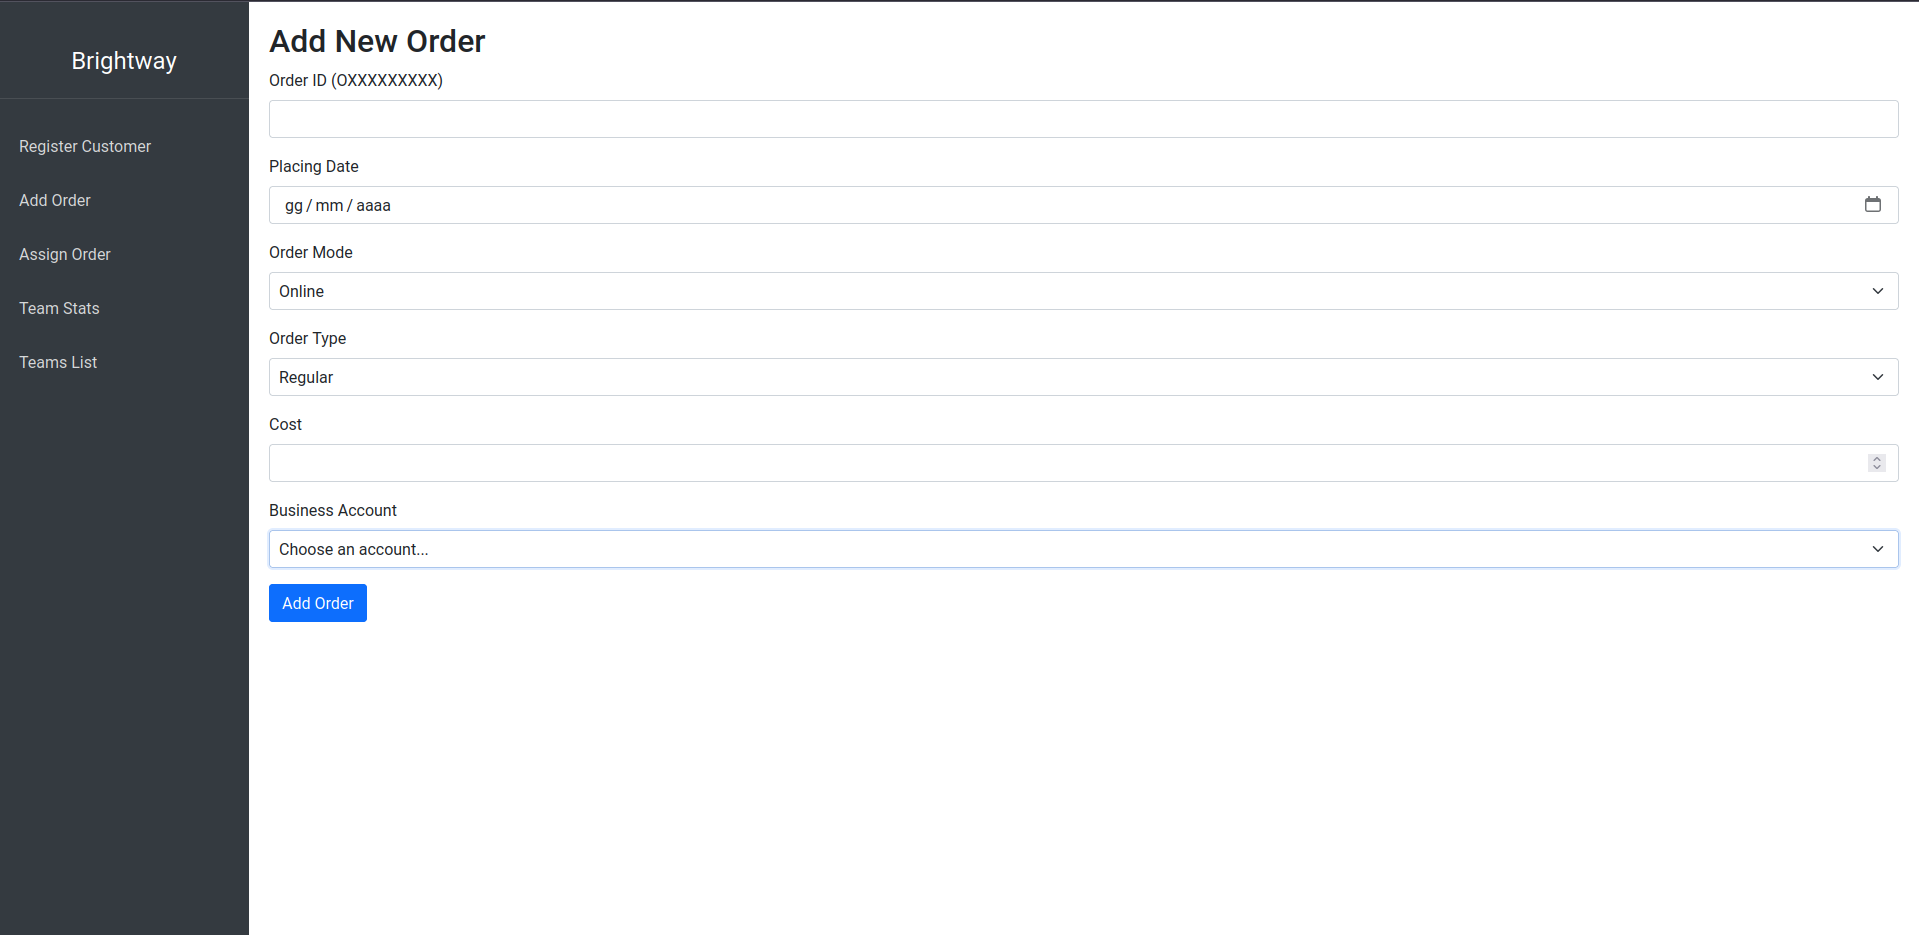
\includegraphics[width=0.8\textwidth]{img/web_app/add.png}
    \caption{Order insertion form.}
\end{figure}

\begin{figure}[H]
    \centering
    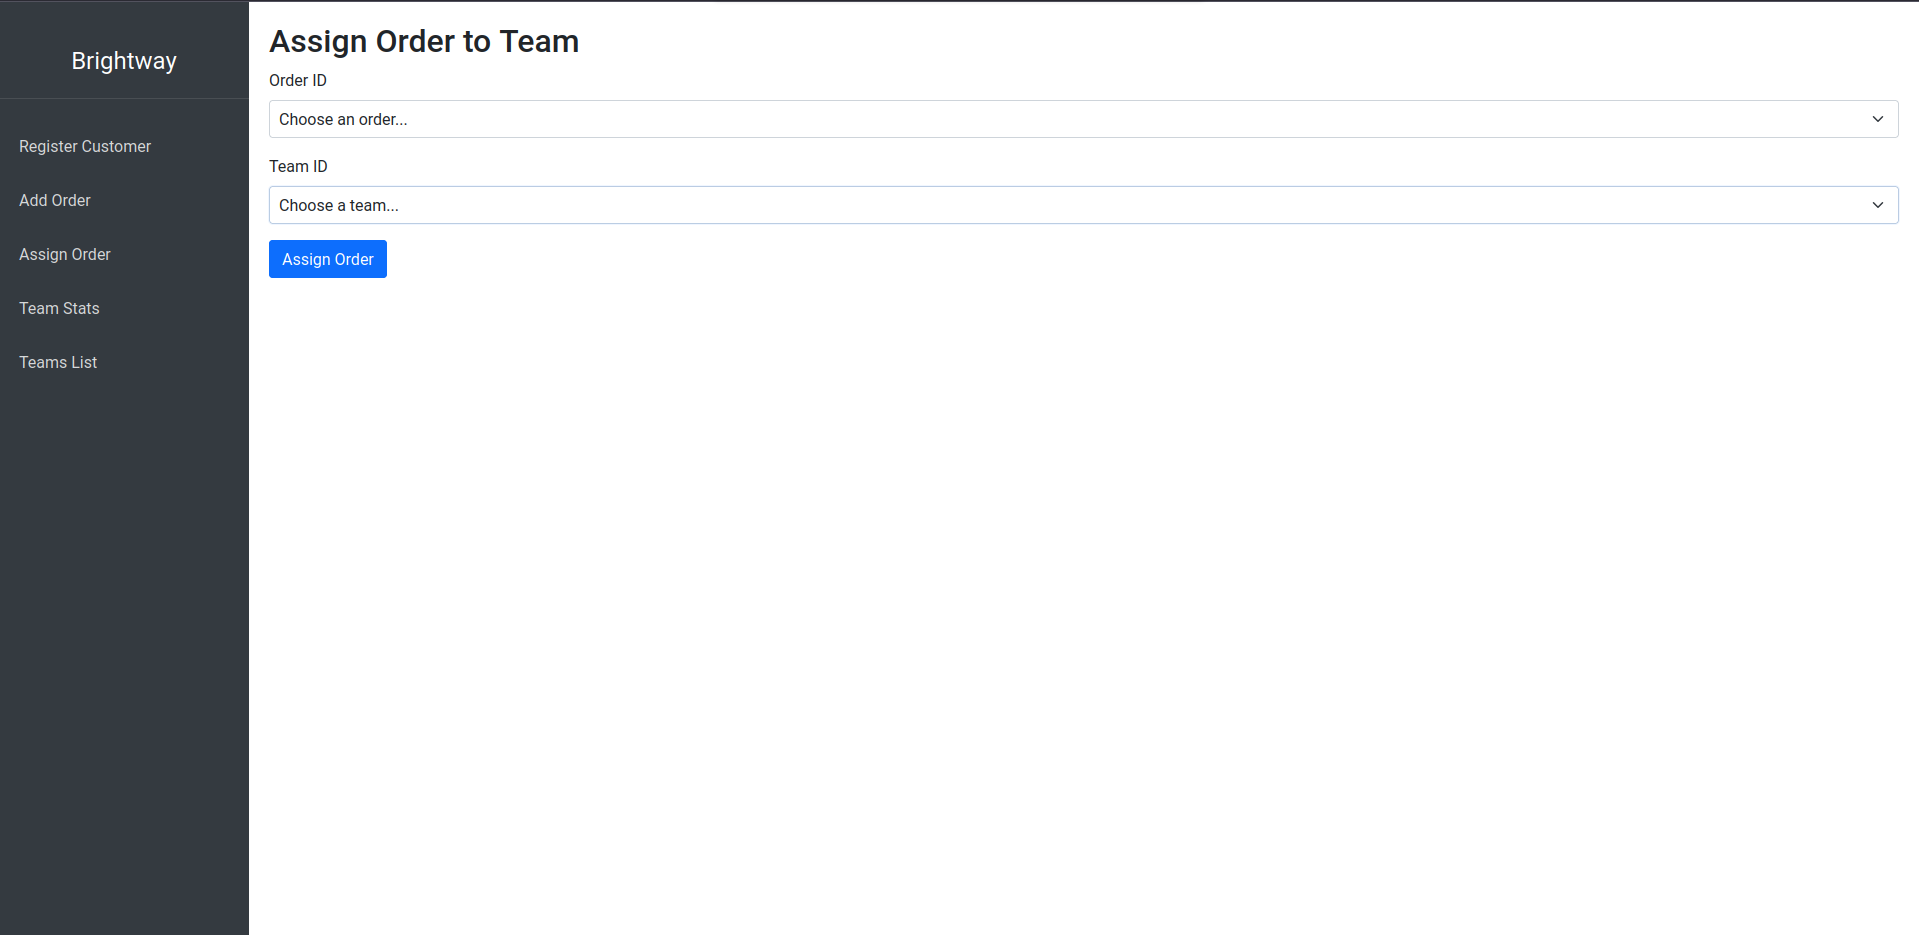
\includegraphics[width=0.8\textwidth]{img/web_app/assign.png}
    \caption{Order assignment form.}
\end{figure}

\begin{figure}[H]
    \centering
    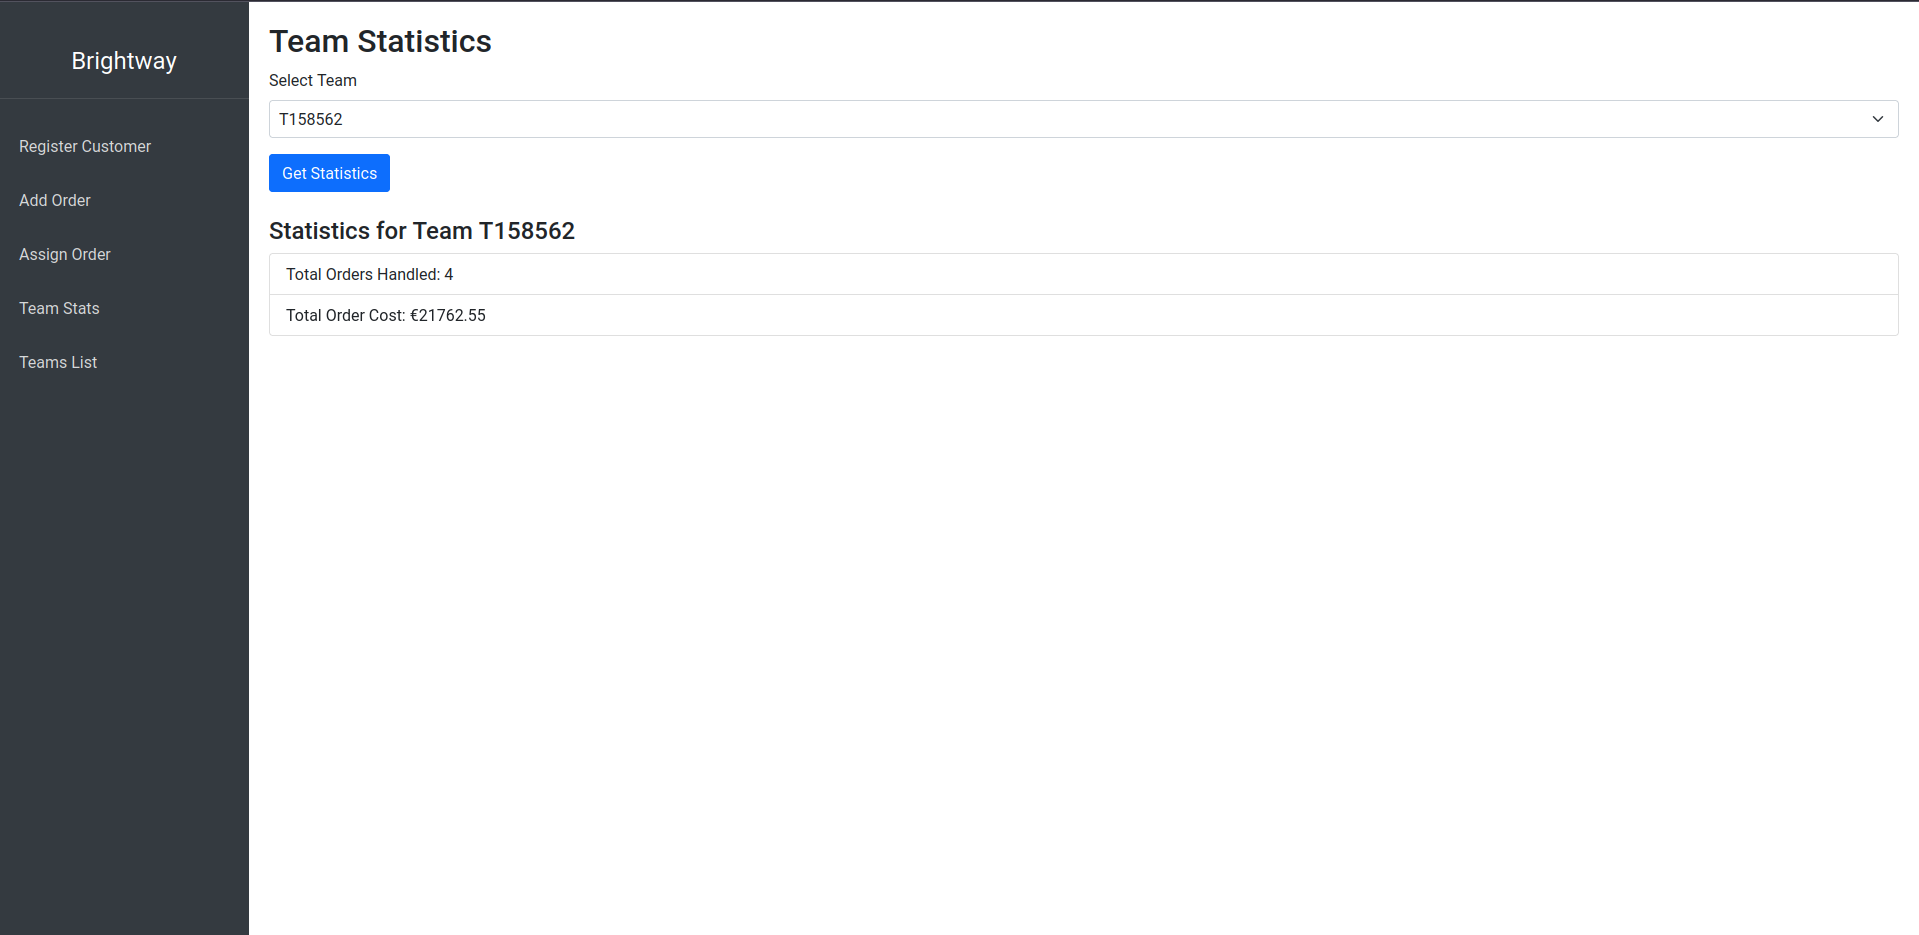
\includegraphics[width=0.8\textwidth]{img/web_app/stats.png}
    \caption{Team statistics page.}
\end{figure}

\begin{figure}[H]
    \centering
    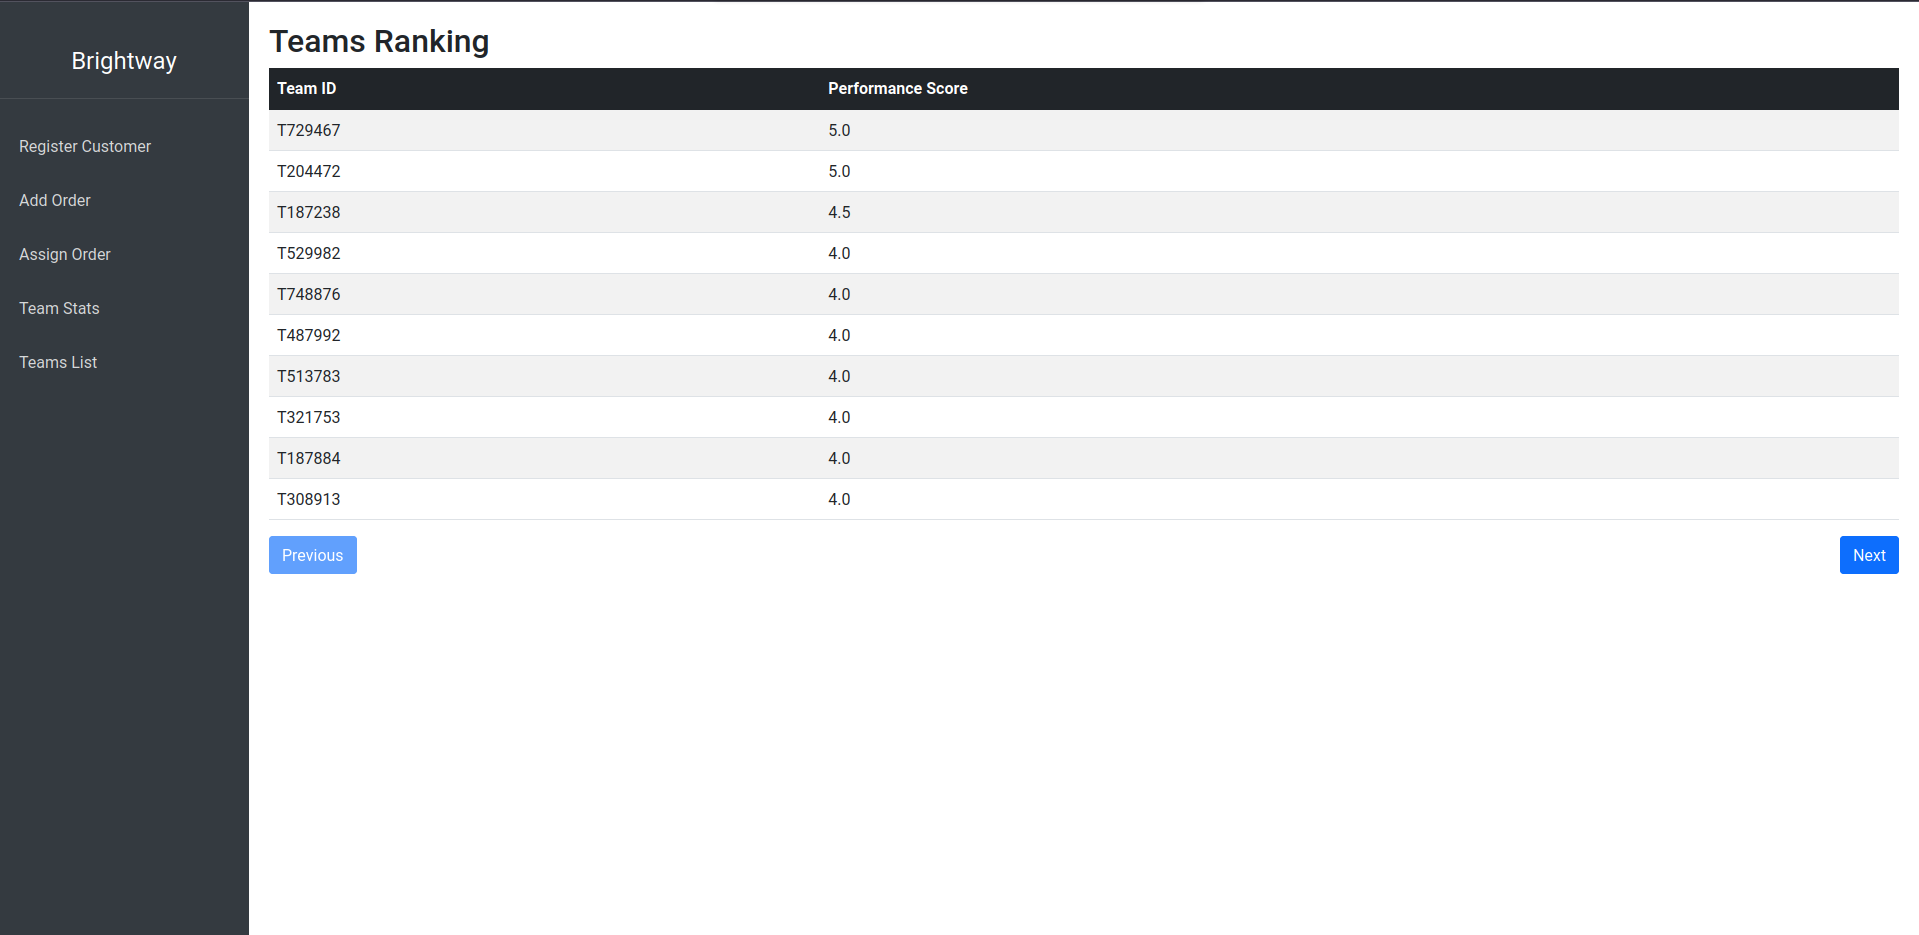
\includegraphics[width=0.8\textwidth]{img/web_app/list.png}
    \caption{List of teams sorted by performance score.}
\end{figure}